\documentclass[11pt, a4paper]{article}

\usepackage{polski}
\usepackage{geometry}
	\geometry{margin = 2.5cm}
\usepackage{indentfirst}
\usepackage{xcolor}
\usepackage{bold-extra}
\usepackage[T1]{fontenc}
\usepackage[utf8]{inputenc}
\usepackage{palatino}
\usepackage{graphicx}
\usepackage[unicode, colorlinks]{hyperref}
\usepackage{fancyhdr}
\usepackage{multirow}
\usepackage{listings}
\usepackage[shortlabels]{enumitem}
	\setlist[itemize]{--, itemsep = 0cm}
\usepackage{amsmath}
\usepackage{subfig}

\linespread{1.3}

\definecolor{codegray}{rgb}{0.5, 0.5, 0.5}
\definecolor{codepurple}{rgb}{0.58, 0, 0.82}
\definecolor{backcolour}{rgb}{0.95, 0.95, 0.92}

\lstdefinestyle{mystyle}{%
	backgroundcolor = \color{backcolour},
%	basicstyle = \ttfamily \small,
 	basicstyle = \ttfamily \footnotesize,
	commentstyle = \color{green!50!black},
	numberstyle = \tiny \color{codegray},
	stringstyle = \color{codepurple},
	keywordstyle = \color{blue!85!black},
	breakatwhitespace = false,
	breaklines = true,
	captionpos = b,
	keepspaces = true,
	showspaces = false,
	showstringspaces = false,
	showtabs = false,
	tabsize = 4,
	numbers = left,
	numberstyle = \tiny \color{black},
	morecomment = [l]{\%},
	frame = single
}

\lstset{
	style = mystyle,
%	language = MATLAB,
	morekeywords = {byte},
	literate = %
		{ą}{{\k{a}}}1
		{Ą}{{\k{A}}}1
		{ć}{{\'c}}1
		{Ć}{{\'{C}}}1
		{ę}{{\k{e}}}1
		{Ę}{{\k{E}}}1
		{ł}{{\l{}}}1
		{Ł}{{\L{}}}1
		{ń}{{\'n}}1
		{Ń}{{\'N}}1
		{ó}{{\'o}}1
		{Ó}{{\'O}}1
		{ś}{{\'s}}1
		{Ś}{{\'S}}1
		{ż}{{\.z}}1
		{Ż}{{\.Z}}1
		{ź}{{\'z}}1
		{Ź}{{\'Z}}1
}

\pagestyle{fancy}
\fancyhf{}
\lhead{WSS -- lab. nr 7 i 8}
%				Numer sekcji????
% \rhead{Sekcja nr 1}
\rhead{Bończyk, Kaźmieruk, Skibiński}
\cfoot{\thepage}

\graphicspath{
	{./img/}
}

%\newcommand{\vectorQ}{$\mathbf{q}$}
%\newcommand{\matrixT}{$\mathbf{T}$}
%\newcommand{\matrixA}{$\mathbf{A}$}
%
%\DeclareMathOperator
%	{\kmPERh}
%	{\textstyle \frac{\text{km}}{\text{h}}}
%\DeclareMathOperator
%	{\mPERs}
%	{\textstyle \frac{\text{m}}{\text{s}}}
%\DeclareMathOperator
%	{\degPERs}
%	{\textstyle \frac{^{\circ}}{\text{s}}}
%\DeclareMathOperator
%	{\radPERs}
%	{\textstyle \frac{\text{rad}}{\text{s}}}
%\DeclareMathOperator
%	{\rad}
%	{\textstyle \text{rad}}
%\DeclareMathOperator
%	{\pitch}
%	{\text{pitch}}
%\DeclareMathOperator
%	{\roll}
%	{\text{roll}}
%\DeclareMathOperator
%	{\yaw}
%	{\text{yaw}}
%
%\setlength{\jot}{0.2cm}


%%%
%%%		DOKUMENT
%%%

\begin{document}



%%%
%%%		TITLEPAGE
%%%

\begin{titlepage}
{\LARGE
\begin{center}
	\begin{figure}[h!]
		\centering
		\includegraphics[width = 0.2\linewidth]{C:/good_folder/nauka/inne/polsl_logo_v2}
	\end{figure}
	
	\vspace{0.25cm}
	
	\textbf{\textsc{Politechnika Śląska}}
	
	\textbf{\textsc{Wydział Automatyki, Elektroniki i Informatyki}}
	
	\vspace{1.5cm}
	
	Wizyjne Systemy Sensoryczne
	
	\vspace{1.5cm}
	
	Lab. nr 7 i 8:
	
	Analiza ruchu w sekwencjach video
	
	\vspace{0.5cm}
	
	{\Large Praca na zajęciach}
\end{center}
}

\vfill

{\Large
\noindent
\textbf{Data laboratorium:} \phantom{0}6.12.2021 r.\\
\phantom{\textbf{Data laboratorium:}} 13.12.2021 r.

\vspace{0.5cm}

\noindent
\textbf{AiR S2-I/Rob}\\
% \textbf{Sekcja nr 1}:
\textbf{Skład sekcji:}

\noindent
\hspace*{0.5cm} Klaudia Bończyk\\
\hspace*{0.5cm} Paweł Kaźmieruk\\
\hspace*{0.5cm} Maksymilian Skibiński\\

% rok 2020/2021, sem. letni, gr. Rob, sekcja nr 1

\vspace{0.5cm}
}

\begin{center}
\phantom{\today{} r.}
\end{center}
\end{titlepage}

\setcounter{page}{2}

\newpage

\section{Wstęp}

W trakcie zajęć laboratoryjnych naszym zadaniem było napisanie programu służącego do obliczania prędkości pojazdów, których ruch został zarejestrowany na zamieszczonych materiałach wideo. Inną propozycją prowadzących było wyposażenie programów w dodatkową funkcję, wyznaczającą zawartość tablic rejestracyjnych wspomnianych pojazdów, której zresztą nie widać. Ostatecznie nie podjęliśmy próby realizacji tego celu i skupiliśmy tylko na celu podstawowym.

\section{Program}

Kod programu został zamieszczony na rysunkach~\ref{fig:main},~\ref{fig:makro1} i~\ref{fig:makro2}.

Program składa się z funkcji \emph{Main} i 4 makrofiltrów:
\begin{itemize}
\item \emph{Odczyt\_Wideo} dla wybranego materiału wideo i numeru klatki początkowej daje na
wyjściu 3 obrazy, które są kolejnymi trzema klatkami wideo.
\item \emph{Top} i \emph{Bottom} służą do lokalizacji geometrycznych środków pojazdów. Jak nazwa wskazuje, jeden z filtrów zajmuje się pasem górnym, a drugi pasem dolnym (dlaczego zostanie wyjaśnione później). Różnią się one jedynie regionem na którym operują filtry.
\item \emph{Points} wyznacza prędkości dla podanych wektorów punktów.
\end{itemize}
Funkcja \emph{Main} poza kontrolą pracy używanych makrofiltrów, zajmuje się także naniesieniem na obraz prędkości.

\subsection*{Makrofiltr \emph{Odczyt\_Wideo}}

Kod tego makrofiltru widoczny jest na rys.~\ref{fig:odczyt}. Jest to najmniej skomplikowany makrofiltr. Jest on używany na samym początku programu. Podajemy ścieżkę do obrazu i numer pierwszej wykorzystywanej klatki wideo. Filtr w środku używa aż trzech funkcji \emph{ReadVideo}, które czytają ten sam materiał wideo, ale odczyt przesunięty jest o jedną klatkę. Nasz program potrzebuje aż odczytywać wideo w ten sposób gdyż:
\begin{itemize}
\item różnica pomiędzy obrazami różniącymi się klatkę wykorzystywana jest by usunąć nieruchome tło z obrazu, a pozostawić jadące pojazdy,
\item różnica pomiędzy obrazami różniącymi się klatkę jest także wykorzystywana do wyznaczenia przemieszczenia.
\end{itemize}

\subsection*{Makrofiltry \emph{Top} i \emph{Bottom}}

Te makrofiltry widoczne są na rysunkach~\ref{fig:top} i~\ref{fig:bottom} i jak już zostało wspomniane różnią się tylko parametrami jednego bloku (1. \emph{CreateBoxRegion}), być może zatem dałoby się to jakoś zamknąć w jednym makrofiltrze, w którym jednym z argumentów byłaby informacja o wybranym filtrze.

\begin{enumerate}
\item Makrofiltr odczytuje dwie klatki wideo, które są przesunięte o jedną klatkę. Wyznaczana jest ich różnica, by usunąć tło z obrazu, a pozostawić pojazdy, które przemieściły się w tym czasie.
\item Następnie używamy progowania dynamicznego do znalezienia krawędzi. Wykonywane jest to jedynie na obszarze wskazanym poprzez \emph{CreateBoxRegion}. Obszar ten wskazuje jeden z pasów na jezdni. Pas ten jest poszerzony tak by samochody po nim jadące znalazły się w regionie w całości i nie stykały się z jego granicami.
\item Na regionie korzystamy z morfologicznego domknięcia, by usunąć drobne nic nie znaczące fragmenty, a jednocześnie domknąć fragmenty istotne tzn. jadące pojazdy. Operacja ta wykonywana jest niesymetrycznie -- elipsa będąca jądrem jest 5-krotnie dłuższa wzdłuż osi poziomej.
\item Region jest dzielony na osobne podregiony, a małe regiony zostają usunięte. Powinny być to nieistotne pozostałości po poprzednich przekształceniach.
\item Regiony, które jeszcze żyją na tym etapie trafiają do funkcji, która pozwala żyć tylko tym, które nie stykają się z granicami.
\item Dla tych regionów wyznaczane są środki geometryczne, które zostają wyrzucone na wyjściu i następnie posłużą do obliczenia prędkości.
\end{enumerate}

Regiony stykające się z granicami zostają usnięte, gdyż w przypadku, gdy pojazd wjeżdża lub wyjeżdża z widoku kamery gwałtownie zmienia swój rozmiar, przez co środek geometryczny nie niesie w poprawny sposób informacji o przemieszczeniu. Poza tym pojazdy, które jadą na przeciwnym pasie nie powinny być brane pod uwagę przez ten filtr.

Dlaczego mamy dwa odrębne makrofiltry zajmujące się pasami osobno, a nie jeden duży będzie bardziej jasne przy opisie filtru \emph{Points}.

\subsection*{Makrofiltr \emph{Points}}

Kod widoczny jest na rys.~\ref{fig:points}.

Filtr otrzymuje dwa wektory punktów opisujących położenie pojazdów z chwil różniących się jedną ,,chwilą'' (jedną klatką) i wyznacza na tej podstawie prędkość. Poza prędkość zwraca na wyjściu także wektor punktów, tak by jasne było, którego samochodu dotyczy która prędkość.

\begin{enumerate}
\item W pierwszej kolejności wyznaczamy rozmiary obu wektorów. Jeśli oba są tych samych rozmiarów to \emph{prawdopodobnie} parę kolejnych funkcji nie ma znaczenia, ale nie zawsze tak jest. Z tych rozmiarów wybierany jest mniejszy.
\item Jeśli wektory różnią się rozmiarem to jeden z nich musi zostać skrócony (chyba zawsze o jeden punkt), podczas gdy ten uboższy w punkt/y pozostanie nie tknięty. Za chwilę powrócimy do tego fragmentu.
\item Następnie wyznaczany jest dystans pomiędzy punktami.
\item Dystans ten jest przemnażany przez odpowiednią liczbę, by przejść z różnicy w pikselach na prędkości.
\item Wynik jest zaokrąglany -- niepotrzebujemy takiej dokładności -- i przekształcany na typ string, który zostanie wykorzystany później na etapie nanoszenia prędkości na obraz.
\end{enumerate}

Kluczowa jest pierwsza połowa makrofiltru i to nad nią dumaliśmy przez dłuższy czas. Problem stanowią sytuacje gdy któryś z samochów na poprzedniej klatce jest, a na aktualnej go nie ma (tzn. chodzi o punkty je reprezentujące) albo na odwrót. Wtedy wektory punktów po pierwsze różnią się liczbą punktów, a po drugie -- i to jest najgorsze -- wektory niekoniecznie są \emph{zsynchronizowane}, te same indeksy dotyczą innych pojazdów.

Synchronizacja wektorów była dla nas bardzo trudna. Jesteśmy zupełnie pewni, że bylibyśmy sobie łatwo poradzić z tym zadaniem w MATLABie czy C, gdzie dobrze potrafimy wykonywać operacje na tablicach i korzystać z pętli. W tym środowisku nie wszystko jest dla nas na tym etapie wystarczająco jasne.

By dokonać synchronizacji wprowadzamy następujące założenie: samochody na górnym pasie pojawiają się z prawej strony, a znikają z lewej, natomiast samochody na dolnym pasie na odwrót. Założenie to jest całkiem sensowne, choć w przypadku, gdyby np. któryś z kierowców jechał pod prąd, nasz program nie działałby w założony przez nas sposób i pokazywał wygórowane prędkości%
\footnote{Z drugiej strony, skoro ktoś jedzie pod prąd to może nie powinien nas boleć fakt, że jego prędkość
zamiast pokazać jakąś faktyczną 50 km/h pokaże 1000 km/h? Zawsze można to potraktować jako słuszny alarm i powód do mandatu.
}%
.
Założenie to oznacza, że jeden z wektorów zawsze będzie tracił elementy na początku, a drugi elementy na końcu. By usuwać elementy z końca korzystamy w bardziej zawiły sposób przy pomocy dwukrotnego odwracania zawartości wektorów poprzez \emph{ReverseArray}.

Poza tym, być może ta funkcja mogłaby być lepiej nazwana...

\subsection*{Funkcja \emph{Main}}

Funkcja główna \emph{Main} (rys.~\ref{fig:main}) koordynuje pracę tych wszystkich funkcji i na końcu nanosi wyniki na obraz. Jako że, ze względu na podział programu na pas górny i dolny, otrzymujemy dwa osobne wektory prędkości i punktów są one wpierw łączone poprzez \emph{JoinArrays}.

Warto zwrócić uwagę na jedną rzecz -- na połączenie wyjść makrofiltrów \emph{Top} i \emph{Bottom} z filtrami \emph{Points}. Są one połączone w \emph{odwrotnej} kolejności. Wynika to z omawianych wcześniej założeń i sposobu działania makrofiltru \emph{Points}. W tych wektorach punktów usuwania elementów musi się odbyć w odwrotnej kolejności temu zostało zastosowane widoczne połączenie.

\newcommand{\www}{0.48}

\begin{figure}[p!]
	\centering
	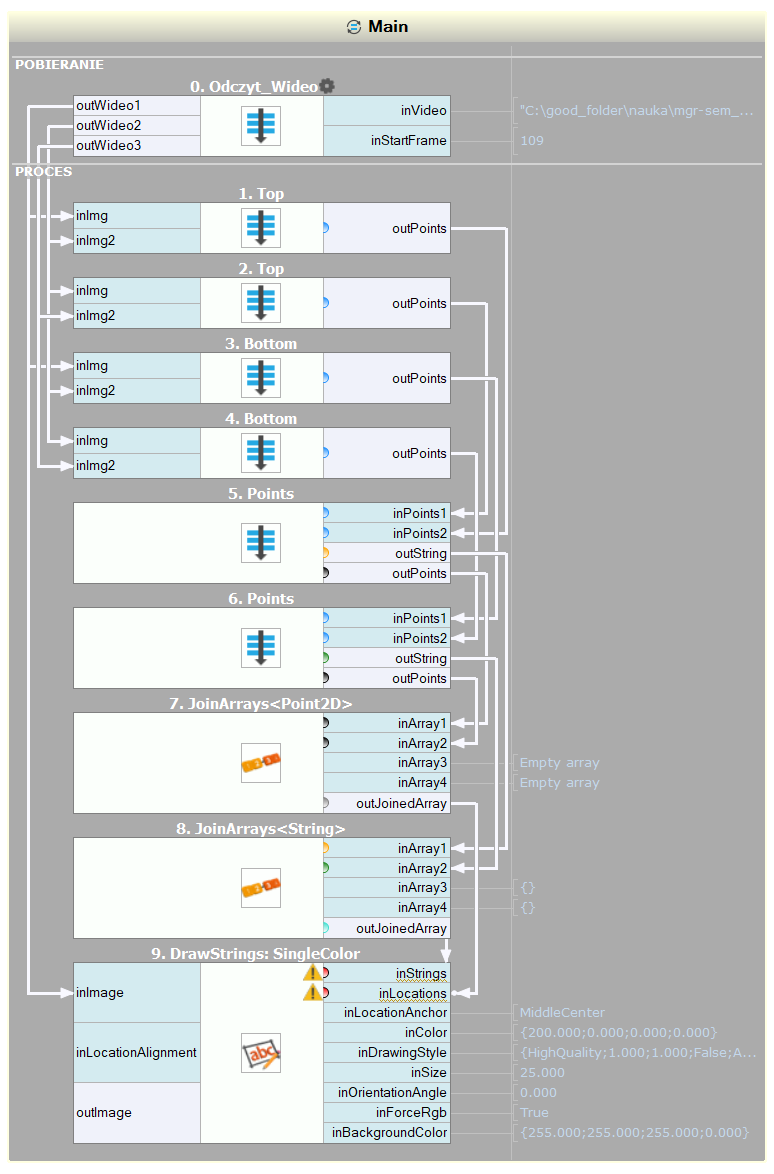
\includegraphics[width = 0.75 \linewidth]{pro1}
	\caption{Funkcja \emph{Main}}
	\label{fig:main}
\end{figure}

\begin{figure}[p!]
	\centering
	
	\subfloat[makrofiltr \emph{Odczyt\_Wideo}]{%
		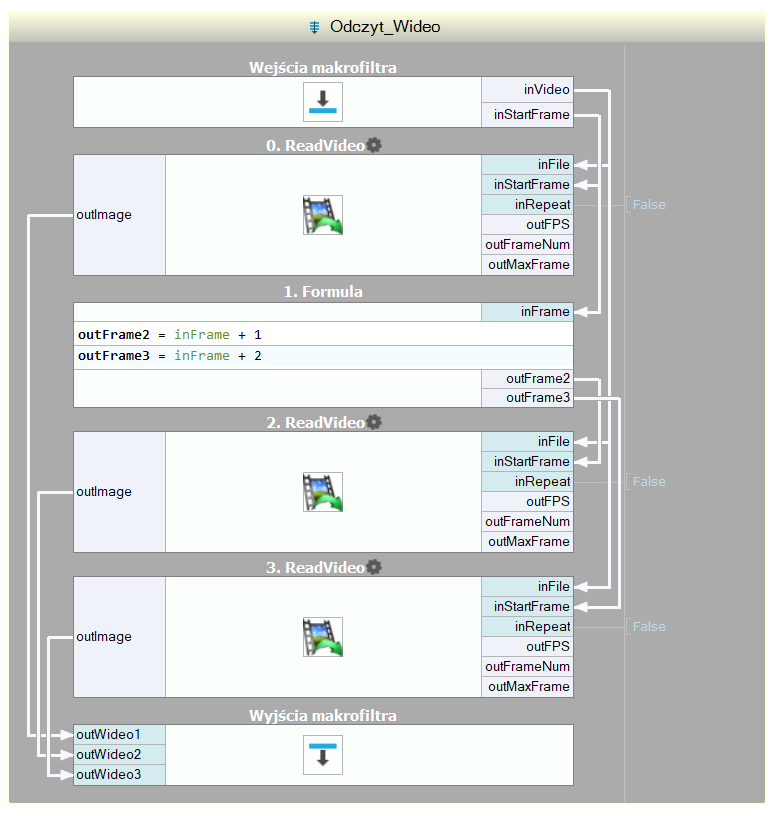
\includegraphics[width = \www \linewidth]{pro3}%
		\label{fig:odczyt}%
	}%
	\hfill%
	\subfloat[makrofiltr \emph{Points}]{%
		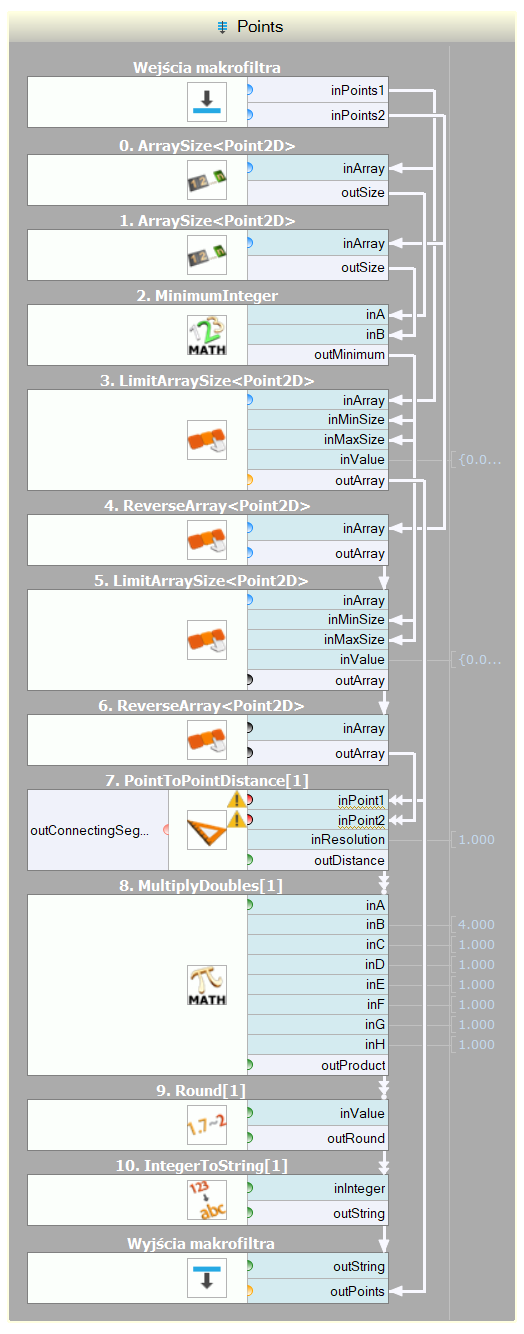
\includegraphics[width = \www \linewidth]{pro4}%
		\label{fig:points}%
	}%
	
	\caption{Makrofiltry cz. 1}
	\label{fig:makro1}
\end{figure}

\begin{figure}[p!]
	\centering
	
	\subfloat[makrofiltr \emph{Bottom}]{%
		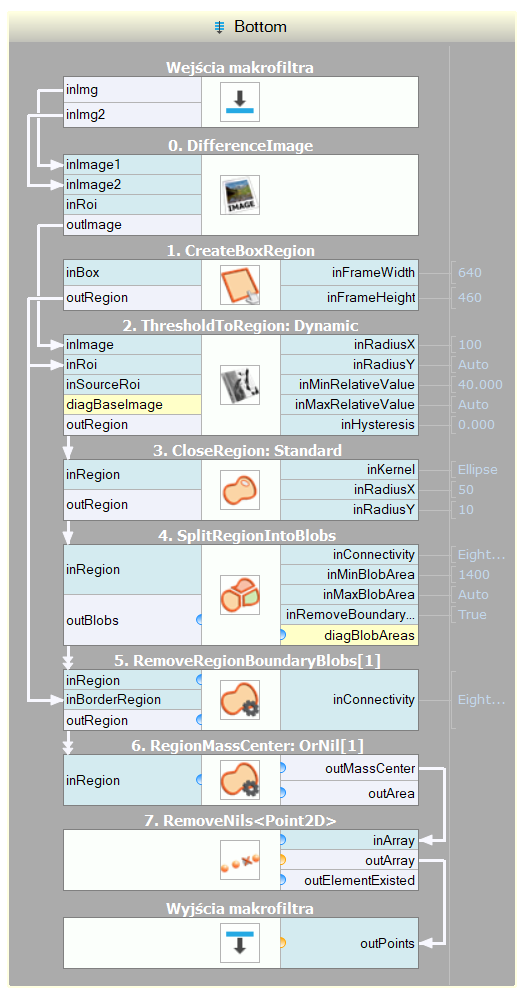
\includegraphics[width = \www \linewidth]{pro2}%
		\label{fig:bottom}%
	}%
	\hfill%
	\subfloat[makrofiltr \emph{Top}]{%
		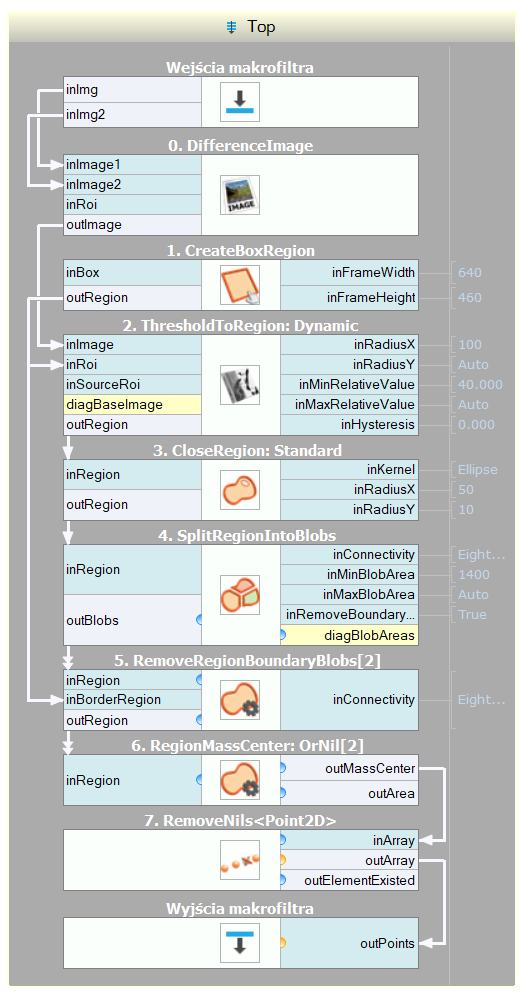
\includegraphics[width = \www \linewidth]{pro5}%
		\label{fig:top}%
	}%
	
	\caption{Makrofiltry cz. 2}
	\label{fig:makro2}
\end{figure}

\clearpage
\newpage

\section{Działanie}

Zacząć można od informacji o tym, że program wyrzuca ostrzeżenia podczas próby uruchomienia go.
\begin{figure}[htbp!]
	\centering
	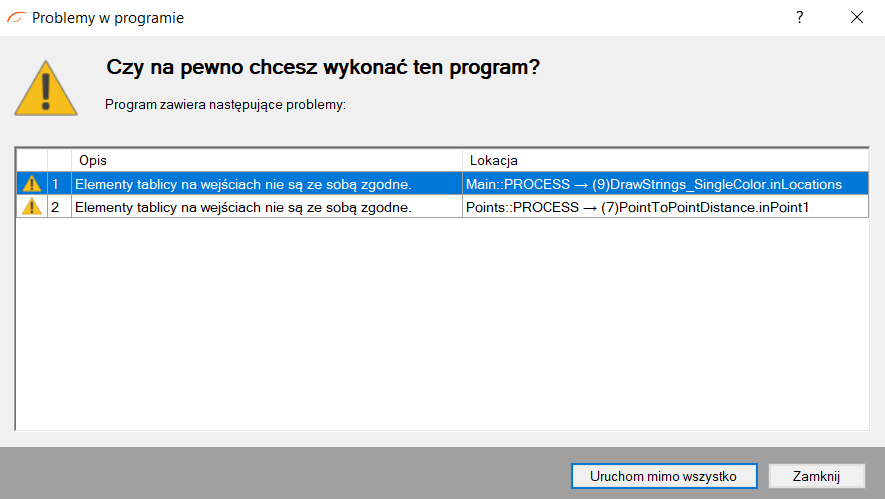
\includegraphics[width = 0.75 \linewidth]{img2}
	\caption{Ostrzeżenie}
	\label{fig:warning}
\end{figure}

Dotyczy ono funkcji wyznaczającej dystans pomiędzy punktami i tej która nanosi prędkości na obraz. Nie udało nam się ani zrozumieć z czego to wynika, ani zauważyć kiedy dochodzi do jakichś problemów. Zignorujmy to.

Działanie naszego programu można ujrzeć na przykładowych obrazach na rysunku~\ref{fig:work}.

\newcommand{\W}{0.32}

\begin{figure}[htbp!]
	\centering
	
	\subfloat[]{%
		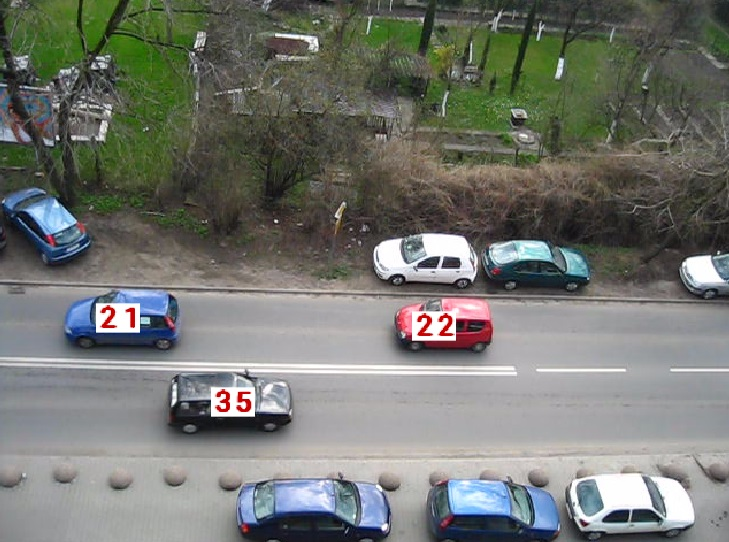
\includegraphics[width = \W \linewidth]{img1}%
	}%
	\hfill%
	\subfloat[]{%
		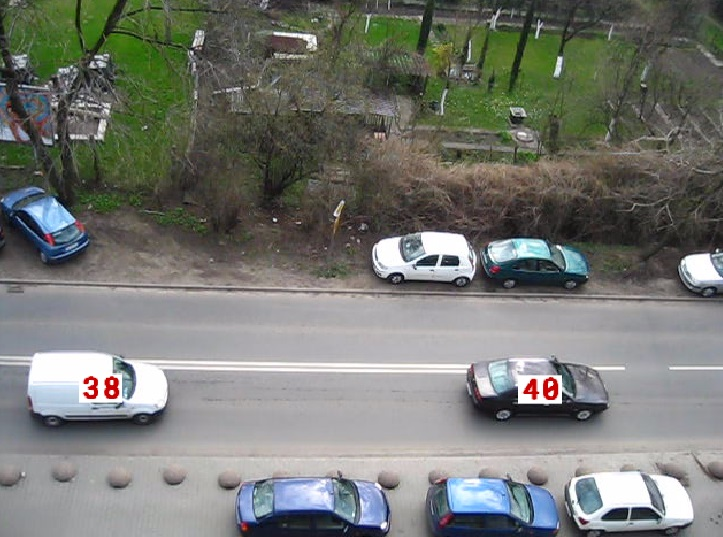
\includegraphics[width = \W \linewidth]{img3}%
	}%
	\hfill%
	\subfloat[]{%
		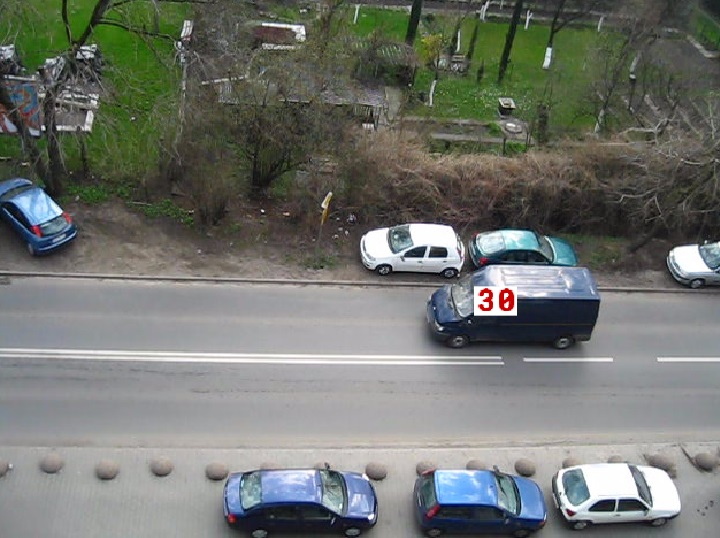
\includegraphics[width = \W \linewidth]{img4}%
	}%
	
	\subfloat[]{%
		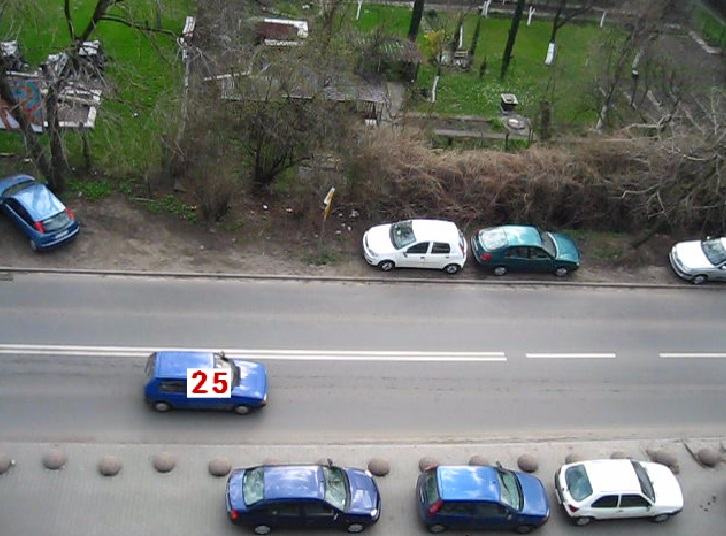
\includegraphics[width = \W \linewidth]{img5}%
	}%
	\hfill%
	\subfloat[]{%
		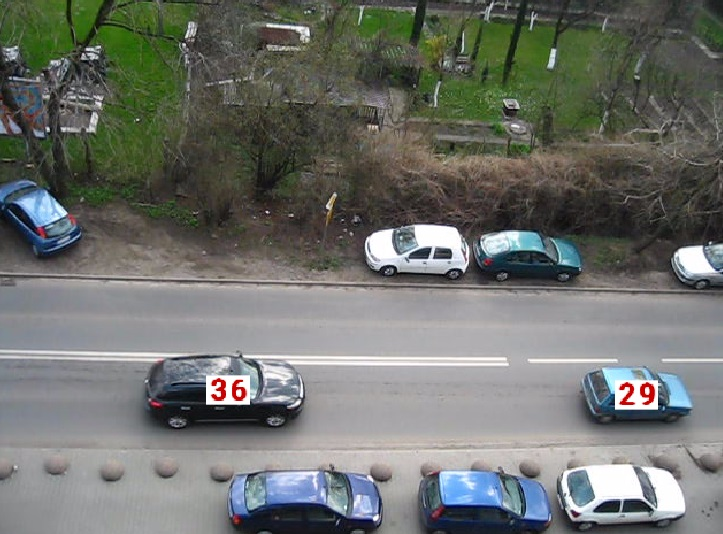
\includegraphics[width = \W \linewidth]{img6}%
	}%
	\hfill%
	\phantom{\subfloat[]{%
		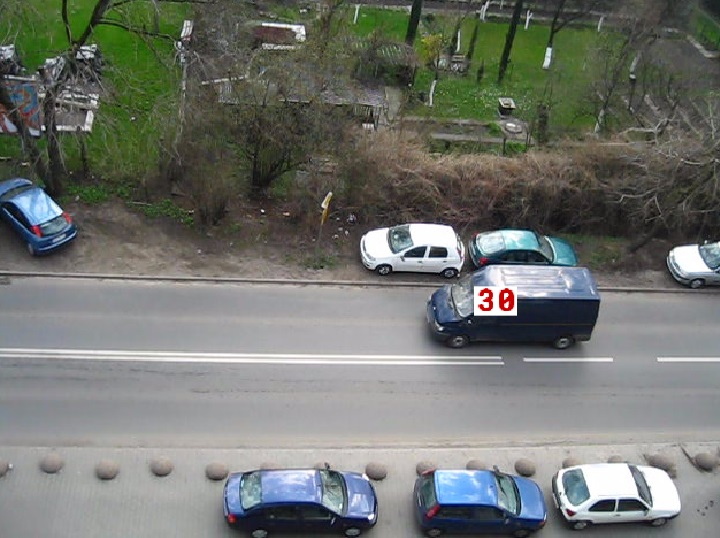
\includegraphics[width = \W \linewidth]{img4}%
	}}%
	
	\caption{Działanie programu}
	\label{fig:work}
\end{figure}

Jak widać gdzieś na jadących samochodach znajduje się informacja o ich prędkości.

Dla mniej skomplikowanych sytuacji np. gdy przejeżdża tylko jeden samochód program działa raczej poprawnie. Pokazuje pewną prędkość, która podlega pewnym zmianom, ale raczej znajduje się na stałym poziomie. Przykładowo trzy kolejne klatki można ujrzeć na rys.~\ref{fig:trzyKlatki}.
\begin{figure}[htbp!]
	\centering
	
	\subfloat[]{%
		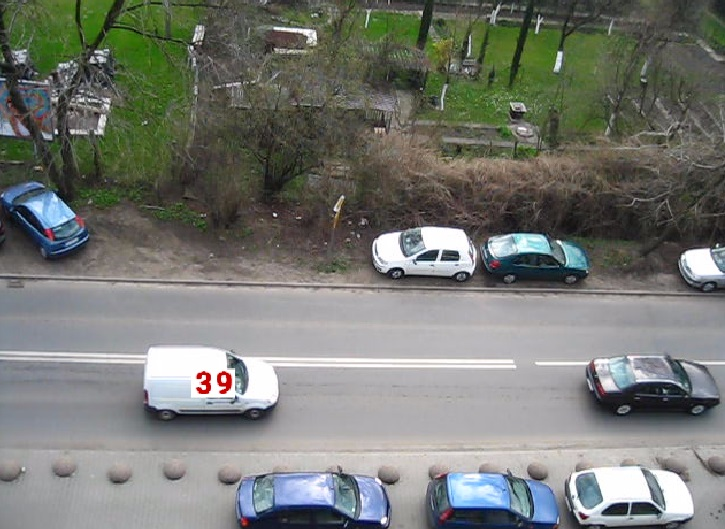
\includegraphics[width = \W \linewidth]{pred1}%
	}%
	\hfill%
	\subfloat[]{%
		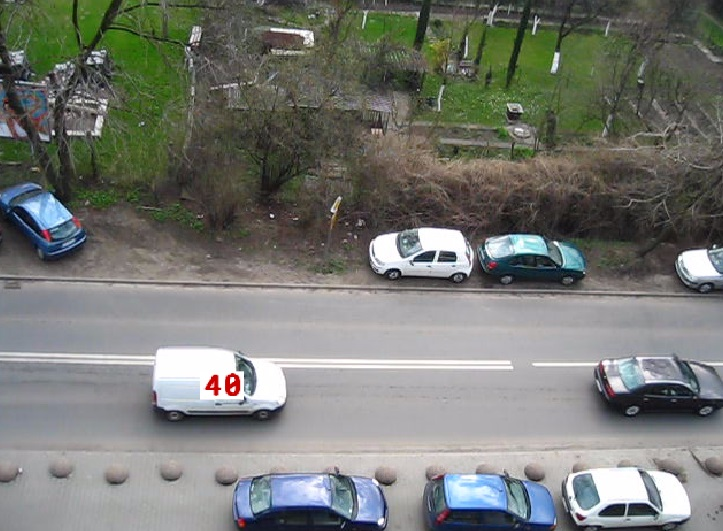
\includegraphics[width = \W \linewidth]{pred2}%
	}%
	\hfill%
	\subfloat[]{%
		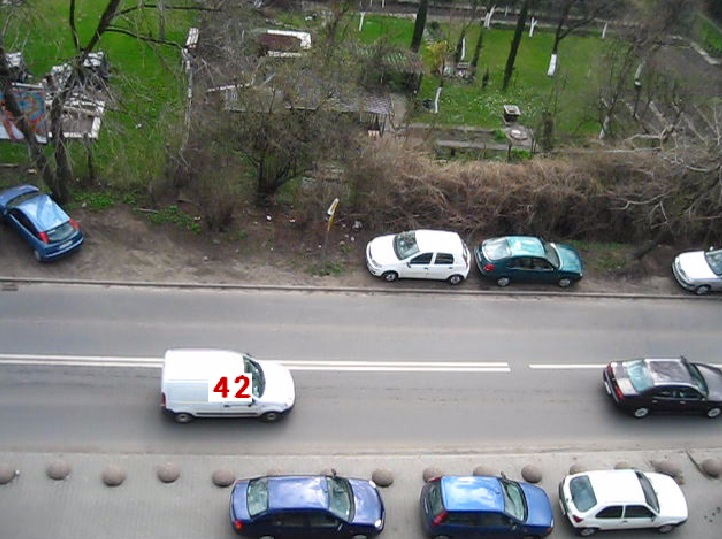
\includegraphics[width = \W \linewidth]{pred3}%
	}%
	
	\caption{Trzy kolejne klatki}
	\label{fig:trzyKlatki}
\end{figure}

Problem stanowić mogą sytuację takie jak:
\begin{itemize}
\item jakiś, nawet drobny, ruch kamery,
\item czasem samochody, które przejeżdżają koło siebie po przeciwnych pasach,
\item czasem samochód, który wyjeżdża z widocznego pola lub wjeżdża na obserwowany część drogi,
\item większe pojazdy mają bardziej ,,skoczną'' prędkość.
\end{itemize}

Możemy teraz streścić kilka z bardziej charaketrystycznych punktów programu.

\subsection*{Pojawiający się pojazd}

Jak już zostało wspomniane dużo czasu zostało poświęcone na poprawną obsługę sytuacji, gdy pojazd pojawia się lub znika. Przykładowa taka sytuacja widoczna jest na rysunku~\ref{fig:poj}.
\begin{figure}[htbp!]
	\centering
	
	\subfloat[]{%
		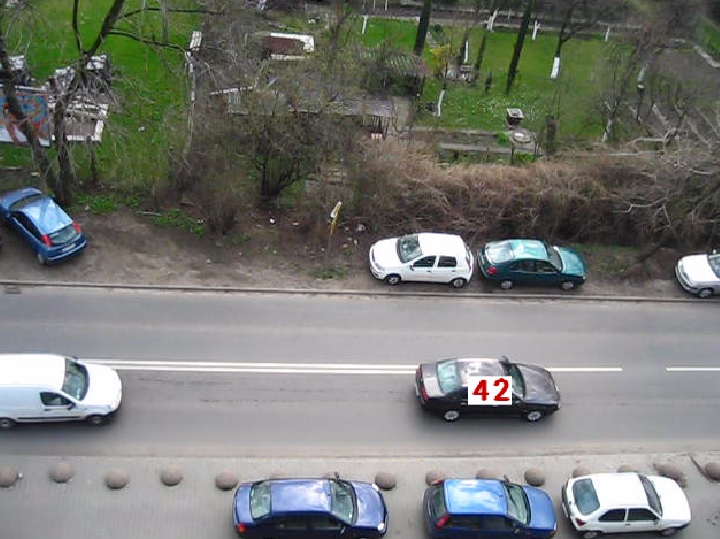
\includegraphics[width = \W \linewidth]{poj2}%
	}%
	\hfill%
	\subfloat[]{%
		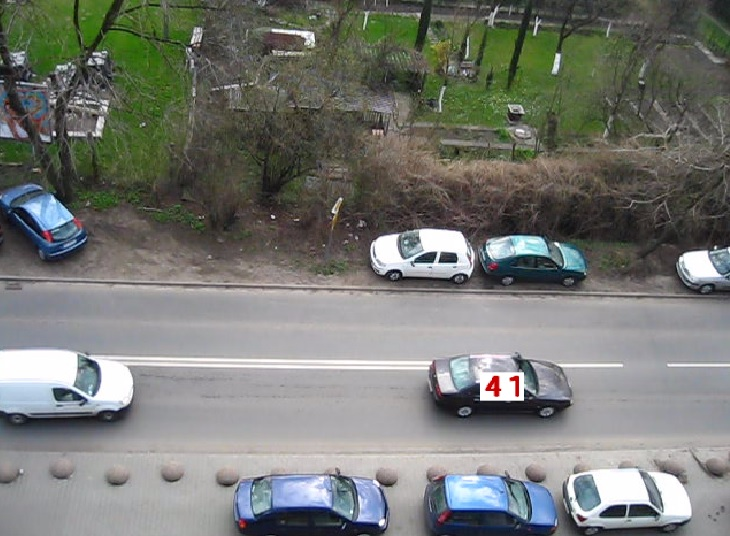
\includegraphics[width = \W \linewidth]{poj3}%
	}%
	\hfill%
	\subfloat[]{%
		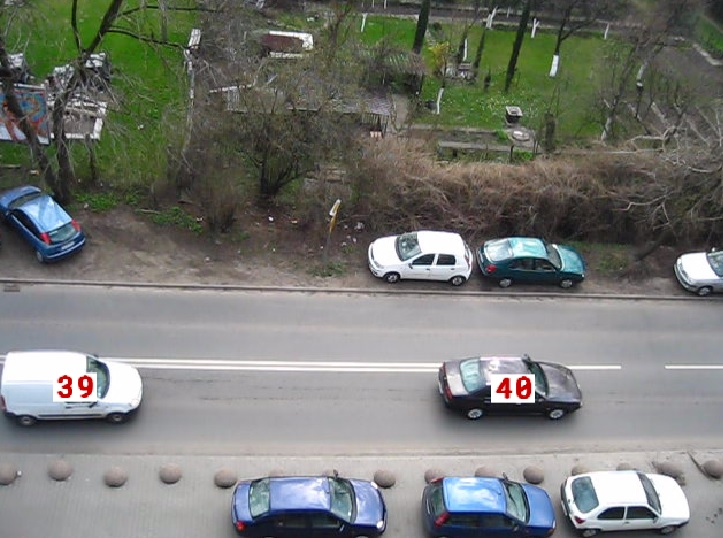
\includegraphics[width = \W \linewidth]{poj4}%
	}%
	
	\caption{Prędkość pojazdu zostaje wyznaczona}
	\label{fig:poj}
\end{figure}

Jak widać nasz trud miał sens, bo udało się coś osiągnąć -- pojawienie się pojazdu nie spowodowało braku synchronizacji pomiędzy wektorami zawierającymi punkty, zatem prędkości obliczane są poprawnie. Ogólnie raczej zawsze tak powinno być, przy spełnieniu wspomnianych założeń o kierunku pojawiających się i znikających pojazdów, ale to się nie zawsze udaje. Problem można zobaczyć na rysunku~\ref{fig:problem1}.
\begin{figure}[htbp!]
	\centering
	
	\subfloat[]{%
		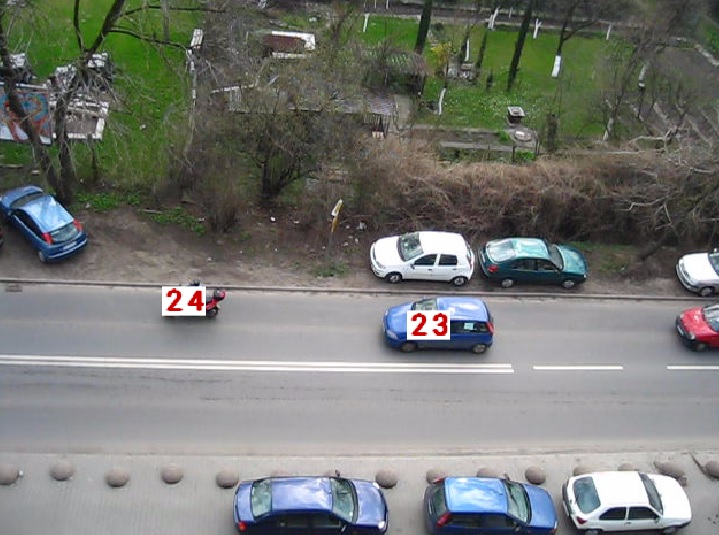
\includegraphics[width = \W \linewidth]{prob1}%
	}%
	\hfill%
	\subfloat[]{%
		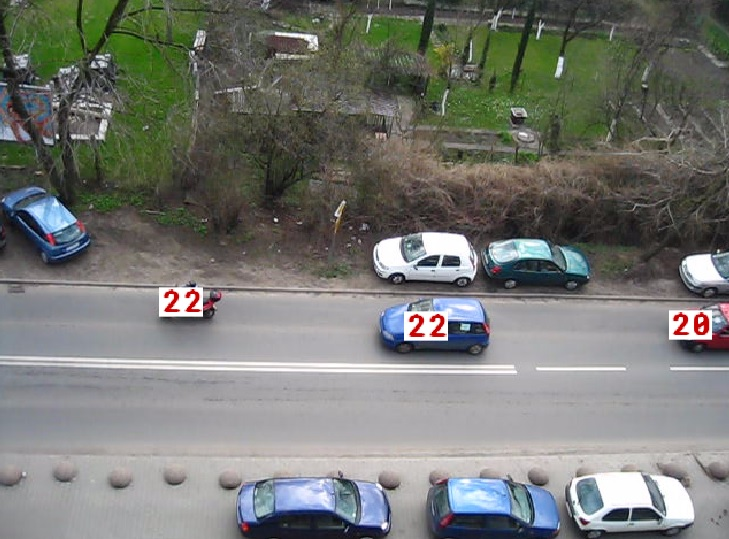
\includegraphics[width = \W \linewidth]{prob2}%
	}%
	\hfill%
	\subfloat[]{%
		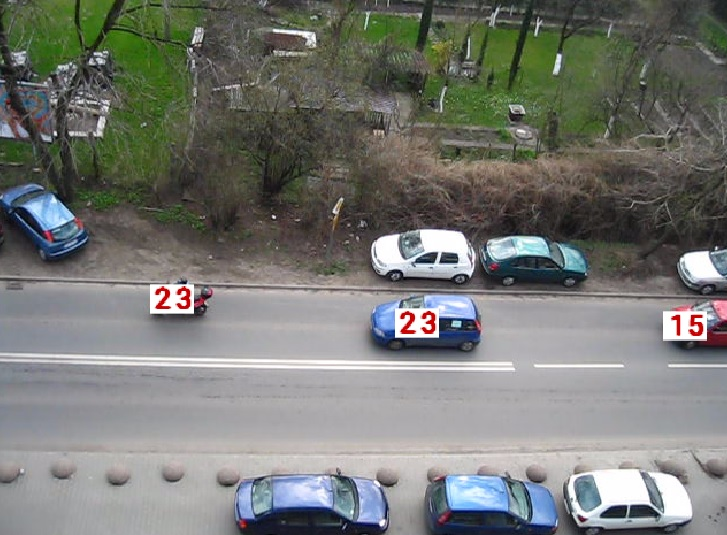
\includegraphics[width = \W \linewidth]{prob3}%
	}%
	
	\subfloat[]{%
		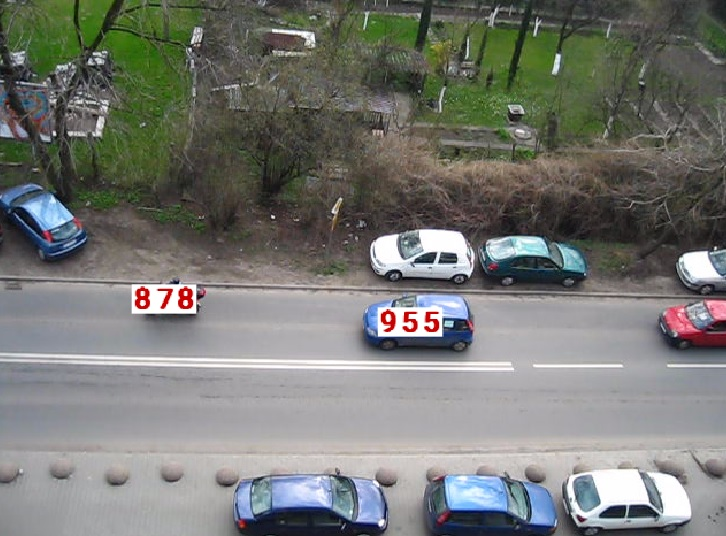
\includegraphics[width = \W \linewidth]{prob4}%
	}%
	\hfill%
	\subfloat[]{%
		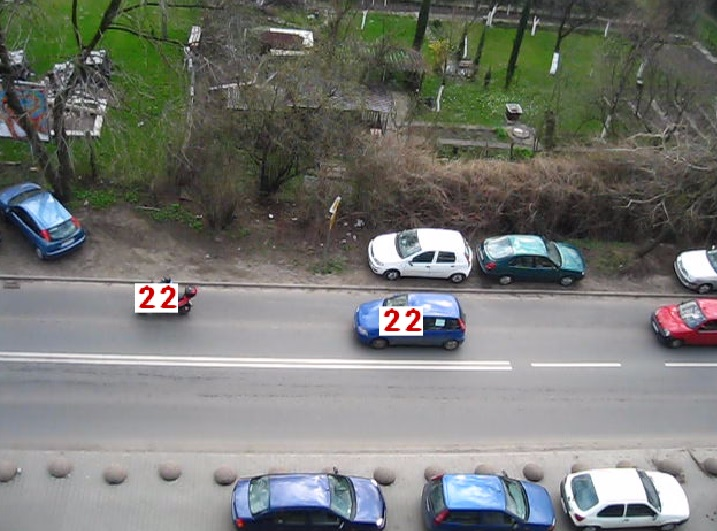
\includegraphics[width = \W \linewidth]{prob5}%
	}%
	\hfill%
	\phantom{\subfloat[]{%
		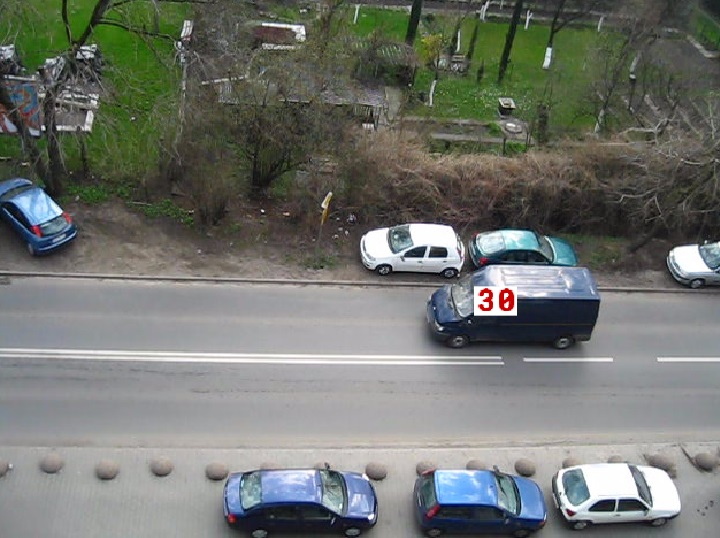
\includegraphics[width = \W \linewidth]{img4}%
	}}%
	
	\caption{Samochód znika w niewłaściwym miejscu}
	\label{fig:problem1}
\end{figure}

Samochód pojawił się z prawej strony, a później znikł (problemy na etapie morfologii -- jedne regiony nie stykają się z granicą, a drugie tak), a przez to wektory przestały być zsynchronizowane na okres jednej klatki i wtedy prędkości gwałtownie skoczyły do bezsensownych wartości. Być może można by je tłumić w takich sytuacjach, ale zaś pojawiłby się wtedy problem poprawnego usuwania odpowiednich punktów/prędkości i punktów wskazujących gdzie na wykresie należy zapisać prędkość.

\subsection*{Chwilowe zniekształcenia}

Czasem zdarzy się, że szum w którymś punkcie wzmocni któreś z krawędzi i niewłaściwy obiekt zostanie potraktowany jako ruchomy pojazd, co widać na rysunku~\ref{fig:skok}.
\begin{figure}[htbp!]
	\centering
	
	\subfloat[]{%
		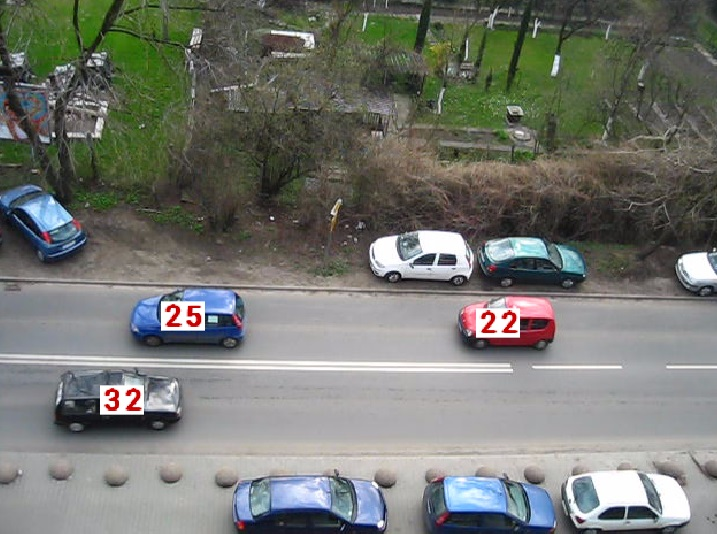
\includegraphics[width = \W \linewidth]{skok1}%
	}%
	\hfill%
	\subfloat[]{%
		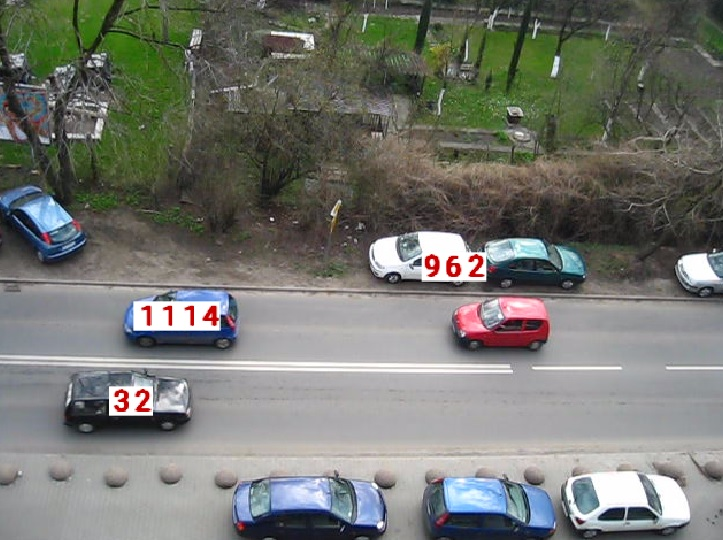
\includegraphics[width = \W \linewidth]{skok2}%
	}%
	\hfill%
	\subfloat[]{%
		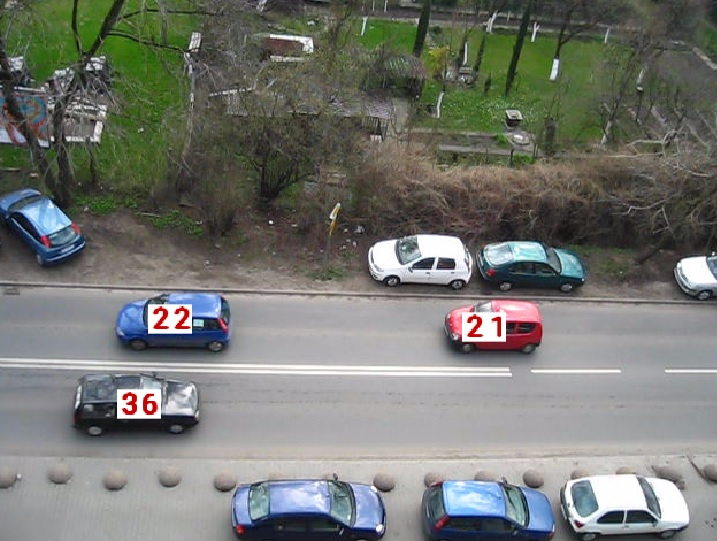
\includegraphics[width = \W \linewidth]{skok3}%
	}%
	
	\caption{Chwilowy skok wartości z powodu wykrycia niewłaściwego obiektu}
	\label{fig:skok}
\end{figure}

Zaś, poza faktem, że prędkość pojawiła się nie tam gdzie trzeba, to wartości gwałtownie skoczyły ze względu na niespełnienie założeń o kierunku znikania i pojawiania się pojazdów.

\subsection*{Omijające się pojazdy}

Te same klatki wraz z kolejnymi (rys.~\ref{fig:omi}) mogą pokazać działanie programu w przypadku gdy pojazdy się mijają.
\begin{figure}[htbp!]
	\centering
	
	\subfloat[]{%
		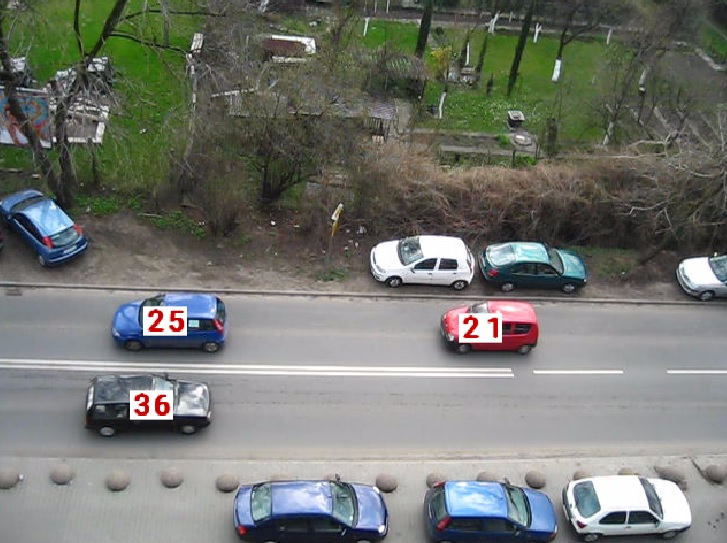
\includegraphics[width = \W \linewidth]{omi1}%
	}%
	\hfill%
	\subfloat[]{%
		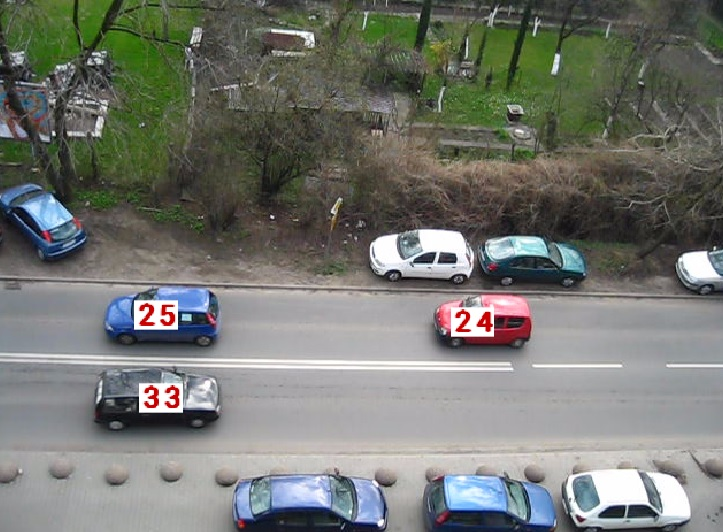
\includegraphics[width = \W \linewidth]{omi2}%
	}%
	\hfill%
	\subfloat[]{%
		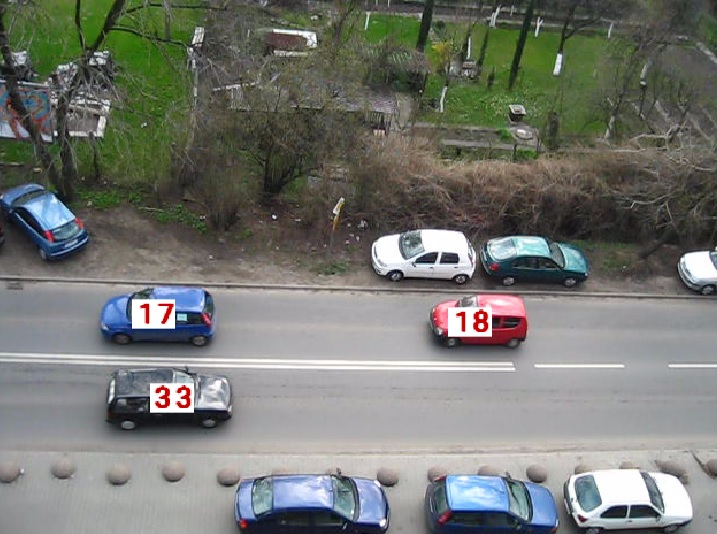
\includegraphics[width = \W \linewidth]{omi3}%
	}%
	
	\caption{Omijające się pojazdy}
	\label{fig:omi}
\end{figure}

W tej sytuacji to, że pojazdy się mijają nie wpłyneło na działanie programu. Zdarza się jednak, że wpływ będzie negatywny.
\begin{figure}[htbp!]
	\centering
	
	\subfloat[]{%
		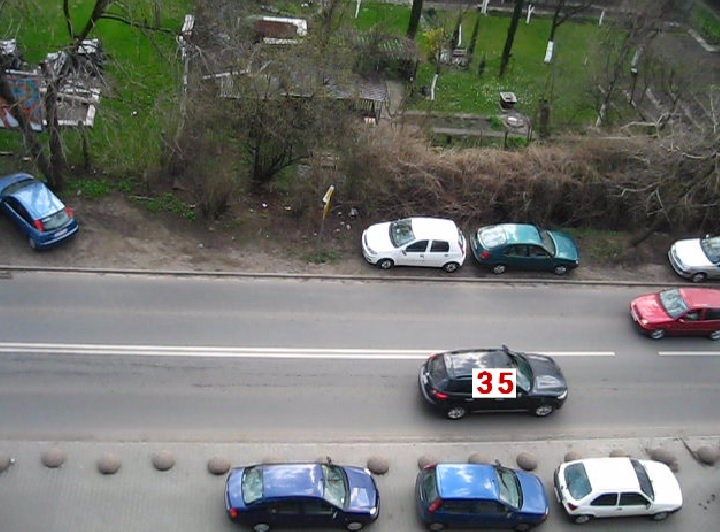
\includegraphics[width = \W \linewidth]{omi_e1}%
	}%
	\hfill%
	\subfloat[]{%
		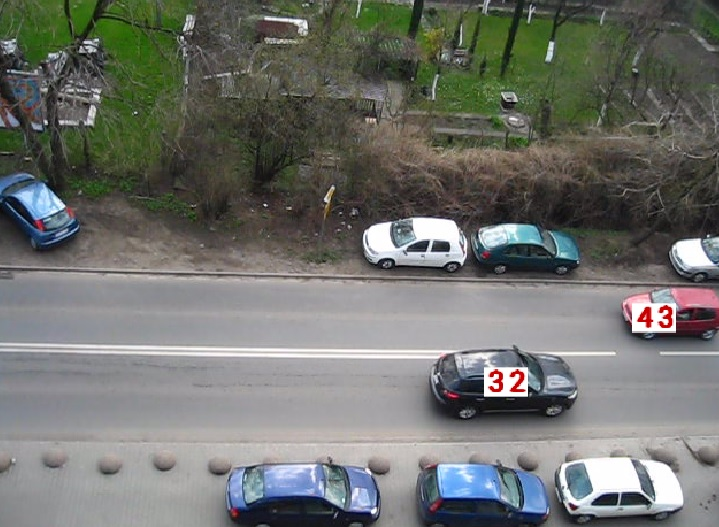
\includegraphics[width = \W \linewidth]{omi_e2}%
	}%
	\hfill%
	\subfloat[]{%
		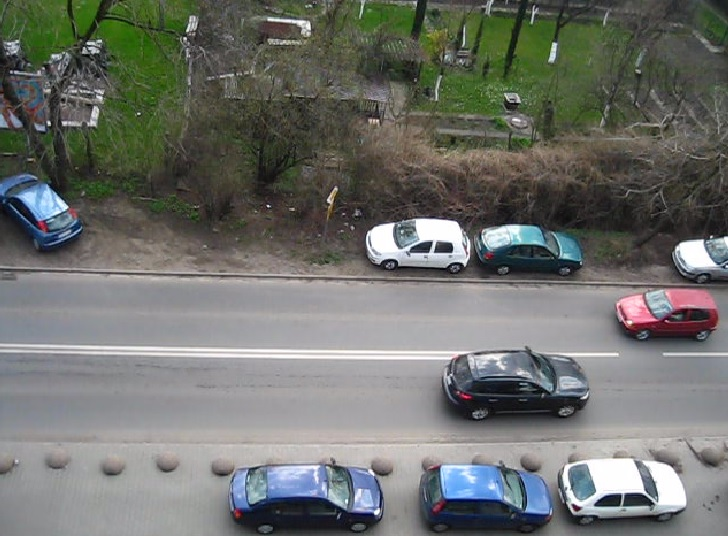
\includegraphics[width = \W \linewidth]{omi_e3}%
	}%
	
	\caption{Omijające się pojazdy -- problem}
	\label{fig:omi2}
\end{figure}

Przykładowo tutaj, spowodowało to, że regiony się zaczęły łączyć i przez to zaczęły się stykać z ustawionymi granicami, zatem ostatecznie regiony te (i tak niepoprawne) znikneły.

\subsection*{Pozostałe}

Poza tym, można wspomnieć, że:
\begin{itemize}
\item Nasz program, mogłyby być lepiej sparametryzowane od strony morfologii czy posiadać inne funkcji na tym etapie. Czasem pomiędzy kolejnymi klatkami regiony reprezentujące jeden pojazd, różnią się wystarczająco mocno, by prędkość skoczył np. z 30 do 60 i potem wróciła. Nie są to tak bolesne skoki jak inne w wyżej omówionych sytuacjach krytycznych, ale są.
\item W przypadku większych pojazdów doszło czasem do tego, że pojazd został rozbity na dwa osobne regiony, albo po tym jak zaczął wychodzić poza obserwowany fragment jezdni (i wypisywana prędkość wraz z nim) nagle pojawia się mniejszy region, który go reprezentuje z jego prędkością. Co prawda z prędkością poprawną, ale i tak widać w tym pewną nie konsekwencję.
\item Kilkukrotnie wspominany problem z synchronizacją mógłby zostać lepiej rozwiązany, ale chyba nie znamy środowiska AVS na tyle dobrze, by wystarczająco zgrabnie operować macierzami.
\end{itemize}

Ogólnie, program działa raczej dobrze i większości sytuacji pokazuje sensowne prędkości.

\end{document}